\chapter[Workshop Connected Minds]{Workshop zur Bestimmung eines Aktionssets}\label{cha:Workshop}
Um ein Konzept für unser Modell abzuleiten, interessiert uns welche Arten von Interaktionen, in einem Auto stattfinden und aus welchen Einzelschritten diese bestehen.
Darüber hinaus wollen wir aktuelle und mögliche Umsetzungen der Modalitäten Haptik, Touch, Sprache und Gestik zu den Einzelschritten sammeln.
Die Interaktionen sollen in die Kategorien Kommunikation, Navigation, Medien, Komfortfunktionen und Einstellungen unterteilt werden.

Zu diesem Zweck wollen wir im Rahmen eines Workshops unsere Ziele erarbeiten.
Dafür ist eine Fokusgruppe geeignet, die sich im automobilen Bereich befindet.   
Bei BMW gibt es wöchentlich die Möglichkeit eine Brainstorming Runde (Connected Minds) mit freiwilligen internen Mitarbeitern anzumelden.
Diese Möglichkeit nutzen wir, um unseren Workshop durchzuführen.
Am 24.08.2016 führten wir mit insgesamt neun Teilnehmern unseren Workshop durch. 
Wir bereiteten unsere Ziele vor, die es zu erreichen galt und wie folgt lauten:  
\begin{enumerate}
	\item \textbf{Ziel A:} Anwendungsbeispiele von Interaktionen im Auto sammeln und diese einer der Kategorien zuordnen (Kommunikation, Navigation, Medien, Komfortfunktionen und Einstellungen). Anschließend diese Anwendungsbeispiele in einzelnen Aktionen zerlegen. 
	\item \textbf{Ziel B:} Die Aktionen aus den Anwendungsbeispielen gruppieren und Umsetzungen für die verschiedenen Modalitäten (Haptik, Sprache, Touch und Geste) finden beziehungsweise sammeln.
\end{enumerate}
\section[Ablauf]{Organisation und Ablauf des Workshops}
\begin{figure}[ht]
  \centering
  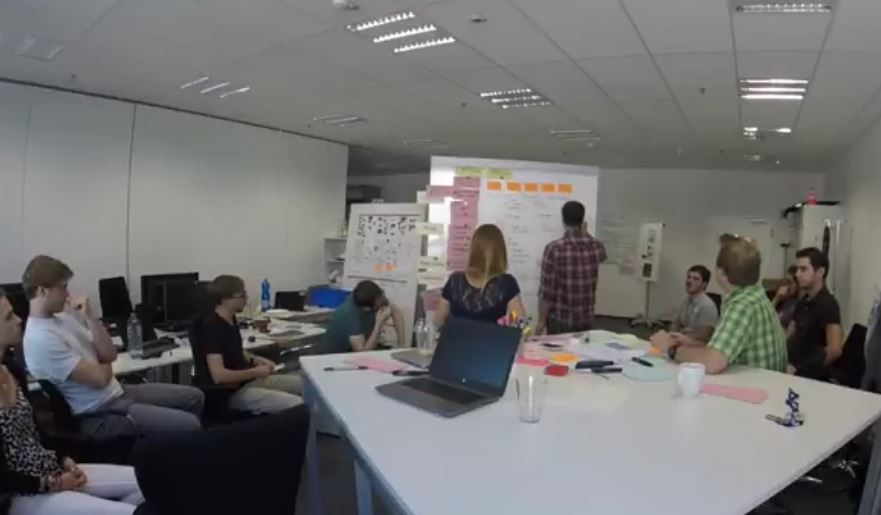
\includegraphics[width=1\textwidth]{img/ConnectedMind.jpg}
  \caption{Connected Minds bei BMW}
  \label{fig:ConnectedMind}
\end{figure} 
Nach einer kurzen Vorstellrunde wurden die Teilnehmer in das Thema eingewiesen und die zwei zu erreichenden Ziele vorgestellt. 
Für das Ziel A sammelten wir im ersten Schritt Anwendungsbeispiele und ordneten sie den Themengebieten Kommunikation, Navigation, Medien, Komfortfunktionen oder Einstellungen zu (siehe \fref{fig:ConnectedMindErgebnisse} linkes Bild). Dazu wurden die Anwendungsbeispiele auf Karten geschrieben und auf einem White-Board in einer Spalte zur passenden Kategorie gepinnt.
\begin{figure}[ht]
  \centering
  \includegraphics[width=1\textwidth]{img/ConnectedMindsErgebnis.jpg}
  \caption[Connected Minds Ergebnisse]{Connected Minds Ergebnisse - Ziel 1 (links), Ziel 2 (rechts)}
  \label{fig:ConnectedMindErgebnisse}
\end{figure}  

Als nächsten Schritt gliederten wir jedes Anwendungsbeispiel in ihre Einzelschritte. 
Diese Einzelschritte sollen Aktionen darstellen, die eine Ebene über den Operatoren eines Keystroke-Level Modells stehen. 
Zum Beispiel würder die Aktion einen Button auszuwählen oder zu drücken, im Keystroke-Level Modell aus einem mentalen Operator, einem Homing Operator und einem Keystroke Operator bestehen. 
Wir betrachten das Auswählen eines Buttons als eine komplette Aktion, die diese Teilschritte enthält. 
Bei der Einteilung der Anwendungsbeispiele in ihre Aktionen achteten wir darauf, dass sie möglichst abstrakt und Interface-unabhängig formuliert werden. 
Ein Beispiel hierfür ist die Abfolge Auswählen, Inkrementieren und Bestätigen.
Alle Aktionen eines Anwendungsbeispiels wurden nacheinander neben das Anwendungsbeispiel geschrieben (siehe \fref{fig:ConnectedMindErgebnisse} linkes Bild). 

Die gesammelten Aktionen wurden für Ziel B gruppiert und auf Karten geschrieben.
Diese Aktionen wurden anschließend auf einem anderen White-Board untereinander gepinnt. 
Für jede Aktion wurden sowohl aktuell bestehende als auch potentiell mögliche Umsetzungen für die Modalitäten Haptik, Touch, Geste und Sprache gesammelt (siehe \fref{fig:ConnectedMindErgebnisse} rechtes Bild und \fref{tab:table1}). 

Der Workshop dauerte insgesamt 1,5 Stunden, davon 30 Minuten für das Erreichen des Ziels A und eine Stunde für das Erreichen von Ziel B. 
Der Workshop wurde auf Video aufgezeichnet.
\section[Ergebnisse des Workshops]{Ergebnisse des Workshops Connected Minds}
Im Workshop wurden insgesamt sechs verschiedene Aktionen identifiziert, aus denen alle Bedienbeispiele zusammengesetzt werden können.
\begin{itemize}
	\item \textbf{Bestätigung (B):} Eingabe oder Auswahl bestätigen.
	\item \textbf{Direktauswahl (DA):} Auswahl aus sichtbaren Elementen.
	\item \textbf{Ein-/Ausschalten (E/A):} Ein- und Ausschalten oder Aktivieren und Deaktivieren von Funktionen.
	\item \textbf{Listen-Navigation (L):} Seitenweise inkrementieren und anschließende Direktauswahl (DA).
	\item \textbf{De-/Inkrementieren (Inkr):} Scrollen, Erhöhen/Verringern von Werten.
	\item \textbf{Texteingabe (T):}  Wiederholte Eingabe eines Buchstabens und anschließende Bestätigung (B).
\end{itemize}

\begin{table}[ht]
	\centering
	\begin{tabular}{|l|l|l|l|l|}
		\hline
		Aktion & Haptik & Touch & Gesten 			& Sprache\\
		\hline
				\multirow {3}{*}{B}
					& Button drücken		& Tap 				& Daumen hoch, 									& Ja,\\
					& Dreh-Drücker			& 						& Tauch OK, 										& OK,\\
					& 									& 						& bestimmte Geste halten 				& passt\\
		\hline
				\multirow{2}{*}{DA}
					& Button drücken		& Swipe  			& 3D-Pointing 								& Objekt/Funktion \\
					& Dreh-Drücker			& Tap					& 														& benennen \\		
		\hline
				\multirow{2}{*}{E/A}
					& Button (on/off)		& Tap,  			& von offener zu 								& Funktionsname\\
					& Kippschalter			& Swipe				& geschlossener Hand						& "`ein"'/"`aus"'\\
		\hline
				\multirow{3}{*}{L}
					& Button drücken		& Swipe				& relative  										& hoch/runter mit\\
					& 									& 						& Handbewegung									& Start/Stop,\\
					& Dreh-Drücker			& Tap 				& (Wischgeste, Swipe), 					& weiter/zurück,\\
					& 									& Scroll			& Drehbewegung des Fingers 			& Tonhöhe variieren\\		
		\hline
				\multirow{3}{*}{Inkr.}		
					& Button drücken		& Swipe				& relative Handbewegung 				& hoch/runter mit\\
					& 									& 						& 															& Start/Stop,\\
					& Dreh-Drücker			& Tap 				& (Wischgeste, Swipe), 					& weiter/zurück,\\
					& Hebel drücken			& Scroll			& Drehbewegung des Fingers			& Tonhöhe variieren\\					
		\hline
				\multirow{3}{*}{T}
					& Tastatur					& X mal Tap 	& In der Luft schreiben, 				& diktieren,\\
					& Dreh-Drücker			& Schreiben		& 3D-Pointing auf Tastatur,			& sprechen\\		
					& Morsecode					& 						& L auf Tastatur								&  \\	
		\hline			
  \end{tabular}
	\caption{Ergebnisse der Umsetzungsmöglichkeiten der Modalitäten für die verschiedenen Aktionen}
	\label{tab:table1}
\end{table}
Für die sechs Aktionen wurden für die Modalitäten Haptik, Touch, Geste und Sprache vorhandene oder mögliche Umsetzungen gesammelt. 
\fref{tab:table1} listet alle Vorschläge der verschiedenen Modalitäten auf.
Wir entschieden uns bei der Modalität mit Touch-Eingabe immer für den direkten Touch auf einem Display. 
Das heißt Buttons und Elemente könnten direkt auf dem Display durch Berührungen bedient werden.
In der schon erwähnten Bachelorarbeit von \citet{stracke2014touch} erwiesen sich diese Variante von Touch-Eingaben für eine gute Umsetzung mit schnellen Interaktionszeiten. 
Auch \citet{Rumelin:2013} bekamen beim direkten Touch die besten Zeiten für das Vollenden einer Aufgabe.

Um den Umfang der geplanten Studie im realistischen Bereich zu lassen, haben wir uns entschieden die Haptik als Modalität nicht miteinzubeziehen. 
Unser Fokus soll bei den Modalitäten Touch, Geste und Sprache liegen, auch weil Haptik im automobilen Kontext bereits in Studien umfassend untersucht wurde \citep{Pettitt_2007, schneegass_2009, SchneegaB_2011}. 
Die haptische Bedienung stellt natürlich weiterhin einen wichtigen Bestandteil der Interaktion im Auto dar.
Da dieser Bereich für uns wegfällt benötigen wir somit die Aktion Ein- und Ausschalten (E/A) nicht. 
Im nicht haptischen Kontext unterscheidet sich diese Aktion nicht von einer gewöhnlichen Aktivierung eines Buttons.

\paragraph{Geeignete Anwendungsbeispiele:}
Aus den im Workshop genannten Beispielen wurden fünf stellvertretende Beispiele identifiziert, die sowohl alle Aktionen abdecken, als auch zu einem der fünf Themengebiete Navigation, Medien, Komfortfunktionen, Einstellungen und Kommunikation zuzuordnen sind. 
\begin{itemize}
\item Navigieren zu "`Rom"', "`Dorfweg"' und "`Kirchengasse"' (Navigation): DA (Navigation) + DA (Zieleingabe) + T (Ziel) + B (Bestätigen)
\item Song "`Happy"' aus beliebten Songs wählen (Medien): DA (Medien) + DA (beliebte Songs) + L ("`Happy"' suchen) + DA ("`Happy"' auswählen)
\item Temperatur um 3 Grad erhöhen (Komfortfunktionen): DA (Temperatur) + Inkr. (+ 3$^\circ$)
\item Lautstärke erhöhen (Einstellungen): DA (Einstellungen) + Inkr. (von 50\% auf ca. 80\%)
\item "`Maria Müller"' aus Kontakten anrufen (Kommunikation): DA (Telefon) + DA (Kontakte) + L ("`Maria Müller"' suchen) + DA ("`Maria Müller"' auswählen)
\end{itemize}
Bei der Einstellung der Lautstärke haben wir uns bewusst für einen groben Zielwert entschieden.
Die Lautstärke soll in ein Intervall zwischen 75\% und 85\% gesetzt werden, da ein genauer Wert (zum Beispiel auf exact 80\% erhöhen) eine unnatürliche Aufgabenstellung wäre \citep{stracke2014touch}. 
Unsere Anwendungsbeispiele stellen übliche Anwendungen dar und sind teils in vereinfachter Weise dargestellt, um eine zu hohe kognitive Belastung zu vermeiden. 
Da die Zeiten von Experten gemessen werden sollen, ist es wichtig Fehler zu eliminieren und Bedenkzeiten zu minimieren.

Die Inkrementation eines Wertes stellen wir in unseren Beispielen in zwei verschiedenen Varianten dar. 
Zum einen soll die Temperatur um 3 Grad erhöht werden, indem durch dreimaliges inkrementieren schrittweise der Wert verändert wird. 
Im anderen Beispiel, die Lautstärke von 50\% auf ca. 80\% zu inkrementieren, wählen wir einen Slider als Darstellung. 
Hier muss nicht eine Aktion 30 mal angewendet werden, um von 50 auf 80 zu inkrementieren, sondern eine direkte Inkrementation (für die Modalitäten Touch und Geste) soll den Wert verändern. 
Wir unterscheiden also zwischen der schrittweisen Inkrementation (Inkr. (s)), die für kleine Wertunterschiede geeignet ist, und der direkten Inkrementation (Inkr. (d)), die bei größeren und gröberen Werteinstellungen vorteilhaft ist.

Bei der Texteingabe eines Ziels haben wir zur Unterscheidung von kurzen und langen Wörtern drei verschiedene Ziele mit unterschiedlicher Länge gewählt ("`Rom"', "`Dorfweg"' und "`Kirchengasse"'). 
Außerdem wurde darauf geachtet möglichst einfach zu schreibende Wörter zu verwenden, um negative Einflüsse in Bezug auf Rechtschreibkenntnissen zu vermeiden. 
Es soll in erster Linie die Zeit gemessen werden, die benötigt wird einen Button bestimmter Größe zu treffen. 
Die mentale Zeit soll sich lediglich auf die Interaktion und das Interface beziehen, nicht jedoch auf auf die Rechtschreibung. 

\section[Idee des Modells]{Abgeleitete Idee für ein multimodales Modell}
Mit unserem Modell sollen sich multimodale Interaktionszeiten vorhersagen lassen, indem sie sich aus den Aktionen Direktauswahl aus sichtbaren Elementen (DA), Bestätigung (B), Listen-Navigation (L), schrittweiser Inkrementation (Inkr.(s)), direkter Inkrementation (Inkr.(d)), und der Texteingabe (T) zusammensetzen.

Bei den Keystroke-Level Modellen auf Operatorebene gibt es eine "`richtige"' Lösung mit einer bestimmten Anzahl an Operatoren. 
Das ist der schnellste Weg, den Experten verwenden, um eine bestimmte Aufgabe zu lösen. 
Bei Interaktionen im Auto ist es deutlich schwieriger eine Abfolge von Operatoren zu bilden. 
Je nach Nutzer und Situation im Auto werden zum Beispiel mehrere Bewegungen vom Lenkrad hin zum Interaktionsbereich gemacht als nötig. 
Deshalb erscheint es uns eine gute Annäherung die Gesamtdauer in unserem Modell nicht durch Operatoren, sondern durch Aktionen zusammenzusetzen. 
Je nach Modalität unterscheiden sich die Zeiten einer Aktion. 

Hinzu kommen Wechselkosten, die auftreten wenn ein Wechsel von einer Modalität zu einer anderen entstehen. 
Auch diese Zeiten gilt es zu berechnen und zu berücksichtigen.
Die Wechselkosten, enthalten unter anderem einen mentalen Operator und einen Homing Operator \citep{Card_1980} bzw. einen Reach Far Operator \citep{Green_2002}. 

Eine Aktion soll in unserem Fall eine durchschnittliche Interaktionsdauer darstellen, die ein geübter Nutzer benötigt in einer bestimmten Modalität die Aktion fehlerfrei auszuführen. 
Wie bei dem KLM soll auch bei unserem Modell von Experten ausgegangen werden. 
Es sollen nur Durchgänge gewertet werden, die keine Fehler vom System oder dem Nutzer mit dem System aufweisen.
Ob ein Nutzer sich dabei Zeit lässt oder einmal mehr oder weniger die Hand vom Interaktionsbereich zurück zum Lenkrad nimmt stellt dabei keinen Fehler dar.
Dies soll in den durchschnittlichen Zeiten berücksichtigt werden.
